\chapter{Further Computational Details}\label{App:Timing}

\section{Comparison of Numerical Routines}\label{App:NumericalRoutines}
Full diagonalization of the Hamiltonian $H$ was performed using the \texttt{eigh} function in NumPy and SciPy. A comparison of the in-built diagonalization routines (Fig. \ref{Fig:Driver_Time_Comparison}) found that the \texttt{evd} driver performed the best, with diagonalization time following the formula:
\begin{equation}\label{Eq:DiagTime}
    t_{\text{diag}}\approx N^3 \times 1.2 \times 10^{-10}\: \text{s}
\end{equation}
Throughout this appendix, $N$ refers to the number of basis states, not the number of particles. For the two-particle, 10$\times$10 unit cell system considered throughout much of this project, $N\approx 4.5 \times 10^4$. As well as the diagonalization of $H$, the eigenstate evolution method (Eq. \ref{Eq:EigenstateEvolution}) also requires a summation of $\mathcal{O}(N^2)$ terms per timestep, with computation time found to be:
\begin{equation}\label{Eq:EigenstateEvolutionTime}
    t_{\text{eig}}\approx N^2 \times 1.1 \times 10^{-8}\: \text{s}
\end{equation}

Evolution in the propagator method (Eq. \ref{Eq:PropagatorEvolution}) was calculated by expressing the Hamiltonian as a sparse matrix, and using the SciPy function \texttt{expm\_multiply}; this far out-performed calculating the exponential using \texttt{expm}, and then separately multiplying it with the state vector. For $J=\hbar=1$, the time for this operation was found to be:
\begin{equation}\label{Eq:PropTime}
    t_{\text{prop}}\approx  N U\Delta t \times 1.0 \times 10^{-6}\: \text{s}
\end{equation}
where $\Delta t$ is the evolution time. The propagator method nearly always performed the best, both due to avoiding the $\mathcal{O}(N^3)$ full diagonalization of the Hamiltonian, and because the cost per timestep is only $\mathcal{O}(N)$, not $\mathcal{O}(N^2)$. In fact, the limiting step with the propagator method was often found to be the $\mathcal{O}(N)$ calculation of observables (such as the density $\langle n \rangle$) from the state $|\Psi\rangle$, not the time-evolution. As the eigenstate method is independent of $\Delta t$ and $U$, it was nevertheless occasionally preferable for certain simulations. Furthermore, the diagonalization only needs to be performed once; thereafter, the eigenvalues and eigenvectors can be used to compute the time-evolution of various initial states.

\vspace{1cm}

\begin{figure}[ht]
    \centering
    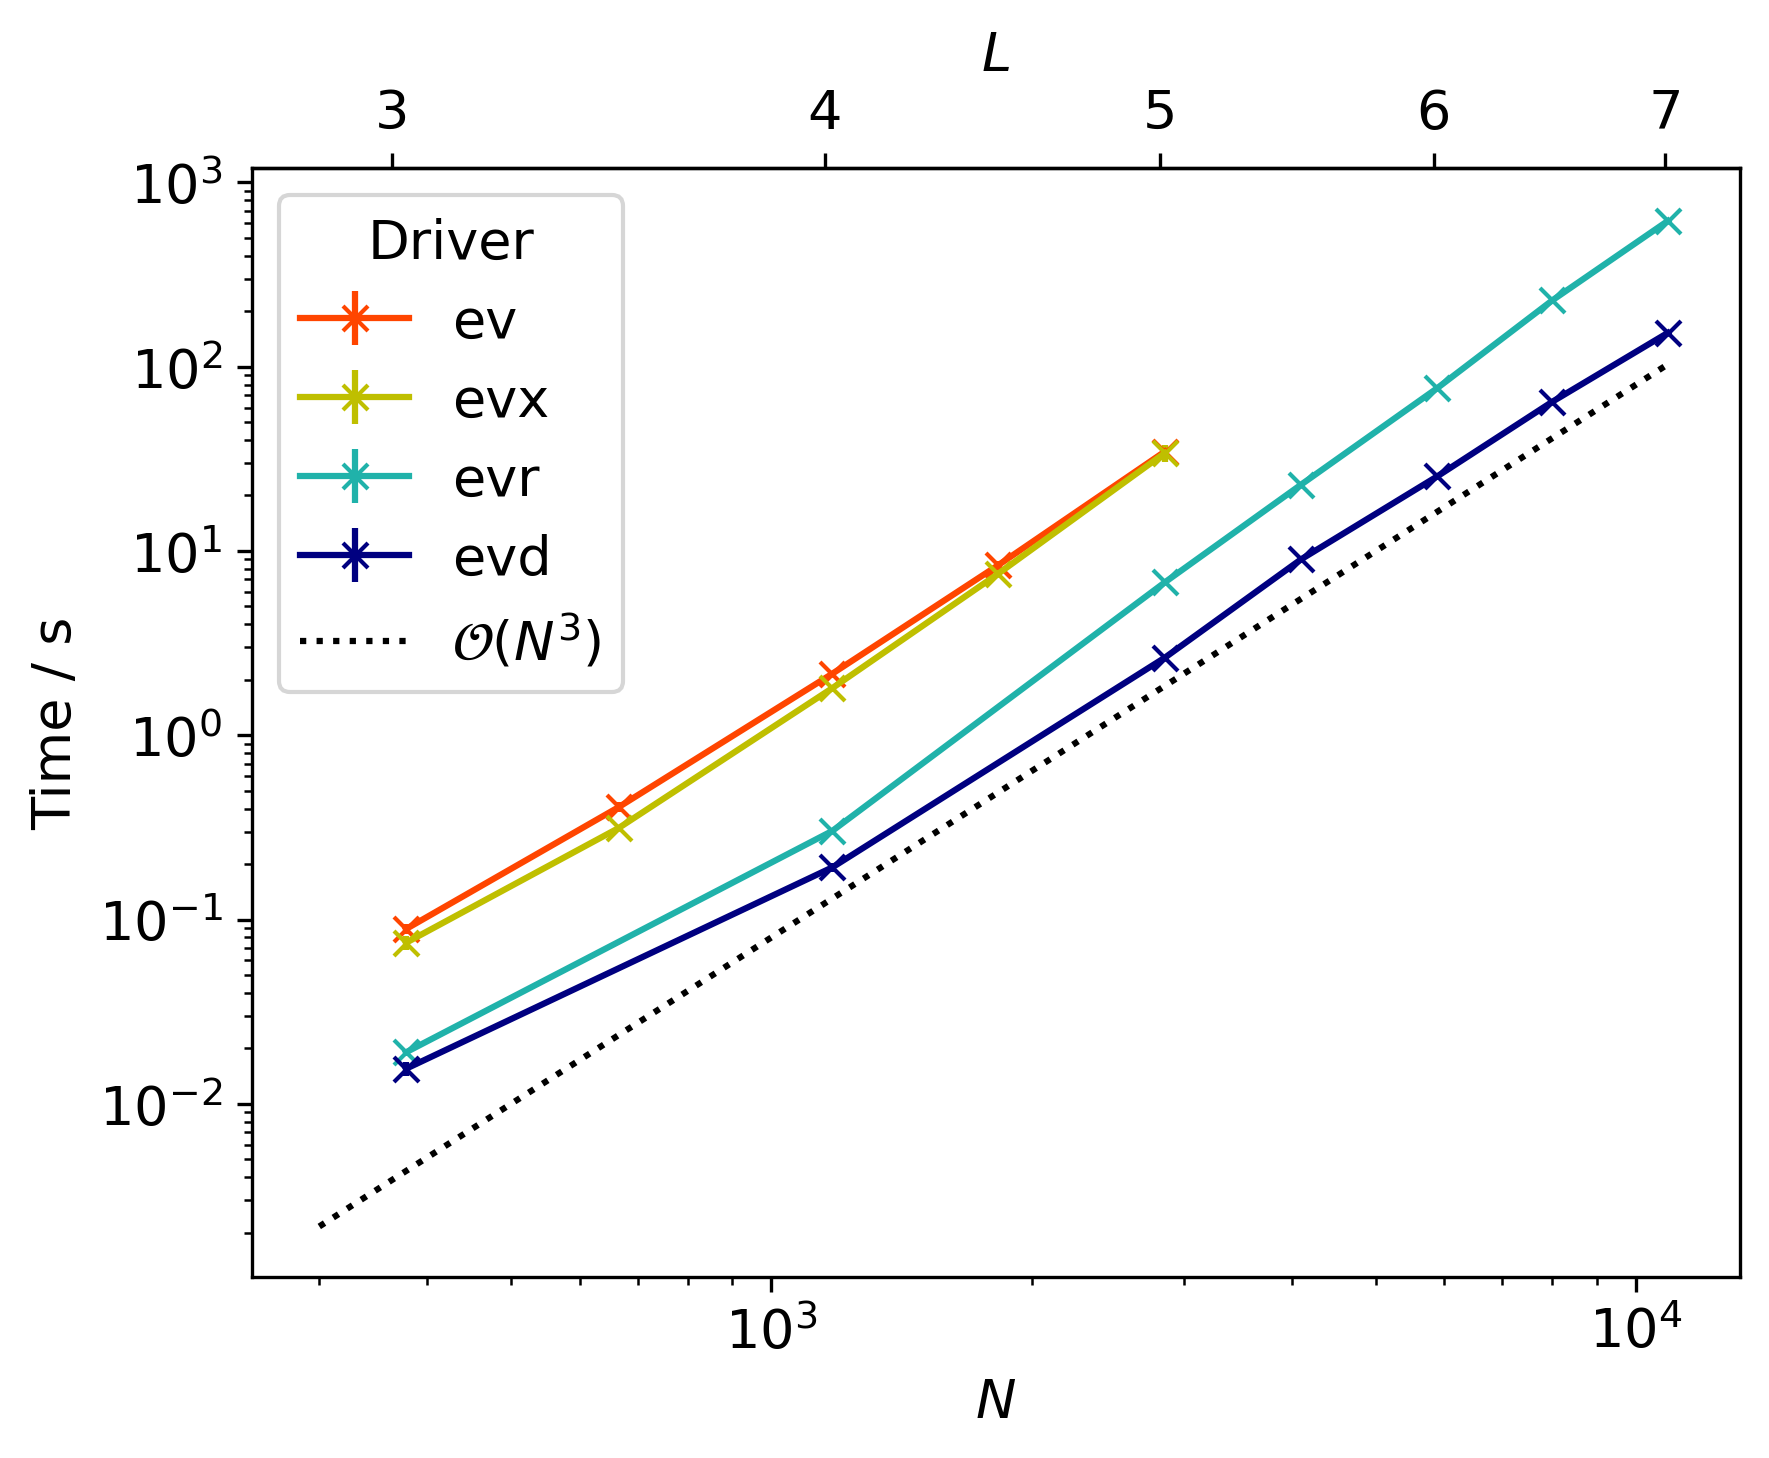
\includegraphics[width=10cm]{Figures/Driver_Time_Comparison}
    \caption{Comparison of computation time for diagonalization of the Hamiltonian matrix, of dimension $N\times N$, for different driver routines. The values of $L$ for which a 2-particle, $L\times L$ unit cell system has $N$ basis states are shown on the upper $x$-axis. The dotted line is a guide to the eye, not the fitted relationship for $t_{\text{diag}}$. Error bars from the random error in repeating the computations are too small to be visible.}
    \label{Fig:Driver_Time_Comparison}
\end{figure}

\newpage

\section{Three-Particle Computation Time}\label{App:ThreeParticle}

To leading order, $N$ scales as $N_{\text{sites}}^{N_A}/N_A!$, where $N_A$ is the number of particles in the system. With the limited computing power and time available for the project, this highly unfavourable scaling with $N_A$ prevented any investigation of systems with $N_A>2$. As a concrete example, for the two-particle system with 10$\times$10 unit cells generally investigated throughout the project, collecting a small dataset such as the one used in Fig. \ref{Fig:Scattering_Evolution} takes $\approx 4$ minutes, with calculating the density the limiting step. Performing an equivalent simulation for a three-particle system would take over six hours; other simulations could be expected to take several days. Performing meaningful research, involving running multiple simulations, was therefore infeasible within the timeframe for the project. Simulations could instead be performed on much smaller systems; 5$\times$5 unit cells would give a similar number of basis states with three particles as 10$\times$10 unit cells with two particles. However, the results of such simulations would likely be severely affected by finite size effects.